\chapter{Design of the testing language}
In this chapter it will be introduced how the tool and the testing language had been designed. The idea was to think of a language that could implement all the possible actions which a security tester would be wanting to do on the messages. One of the objective was to think of a language that could define tests that could then be tested over multiple webservices. For example, a series of tests to verify the well-known vulnerabilities of a specific protocol could be defined and then used on any type of website.
I had to decide how to write and define the tests, I thought I could define a proper language with a dedicated parser, but it was not worth the effort, as there were already some well-tested alternatives available. one of them is JSON, which has been used as a base over which write the tests. JSON is a convinient way of defining gerarchical sturctures like tests are.
The idea behind this language is that a specific message can be intercepted and checked or edited in some way.
The gerarchical structure and the details of the language will be discussed in this chapter.

\section{Test example: PKCE Downgrade}
I want to introduce the language with an example. Due to its complexity, having a real example before the explanation of all its components could be helpful to understand their use.
To understand this test, a brief introduction of PKCE has to be done, as said in \cite{pkce_explanation}: The Proof Key for Code Exchange (PKCE, pronounced pixie) extension describes a technique for public clients to mitigate the threat of having the authorization code intercepted. The technique involves the client first creating a secret, and then using that secret again when exchanging the authorization code for an access token. This way if the code is intercepted, it will not be useful since the token request relies on the initial secret. 
The PKCE Downgrade test has as objective to test an OAuth vulnerability where removing the parameter "code\_challenge" from the url of an authorization request message will be downgrading the authentication proces in a way that PKCE will not be used if the service is vulnerable \cite{pkce_downgrade}. To test this, we have to intercept the authorization request message, remove the parameter "code\_challenge" from it, and then forward it.
The complete test can be found in attachment \ref{chap:PKCE_complete}


% The first Operation defined in this test at line 17 is an operation that is used to start the session (and the browser). The automated browser will execute a series of actions defined by the user in a \gls{session track}. The actions in this case will do a complete login in a website that uses OAuth as SSO login option. During the execution of the actions, language's Operations will be executed. At line 21 there is an Operation used to intercept an "authorization request" message, that is defined in an apoosite file where all Message Types are defined. Once an authorization request message is intercepted, the preconditions at line 32 are executed, checking that the parameter we want to test the vulnerability is used. This is done because the parameter "code\_challenge" is not an optional parameter for the OAuth protocol, so, if it is not present, i want the test to result "not applicable" instead of failed or passed.
% The next part of the example is the Message Operation at line 35, where I tell to remove from the intercepted message's url the "code\_challenge" parameter.
% The last part of the test is the definition of the result, the result is part of the evaluation of a test, in this case it is set to "incorrect flow s1", this means that I want the test to be considered passed if the execution of the session s1 is incorrect that is, if the execution of the session s1 encounters an error or an unexpected page.


\section{Language structure}
Each object of the language is a JSON object which can contain different possible tags based on its type.
\begin{figure}
    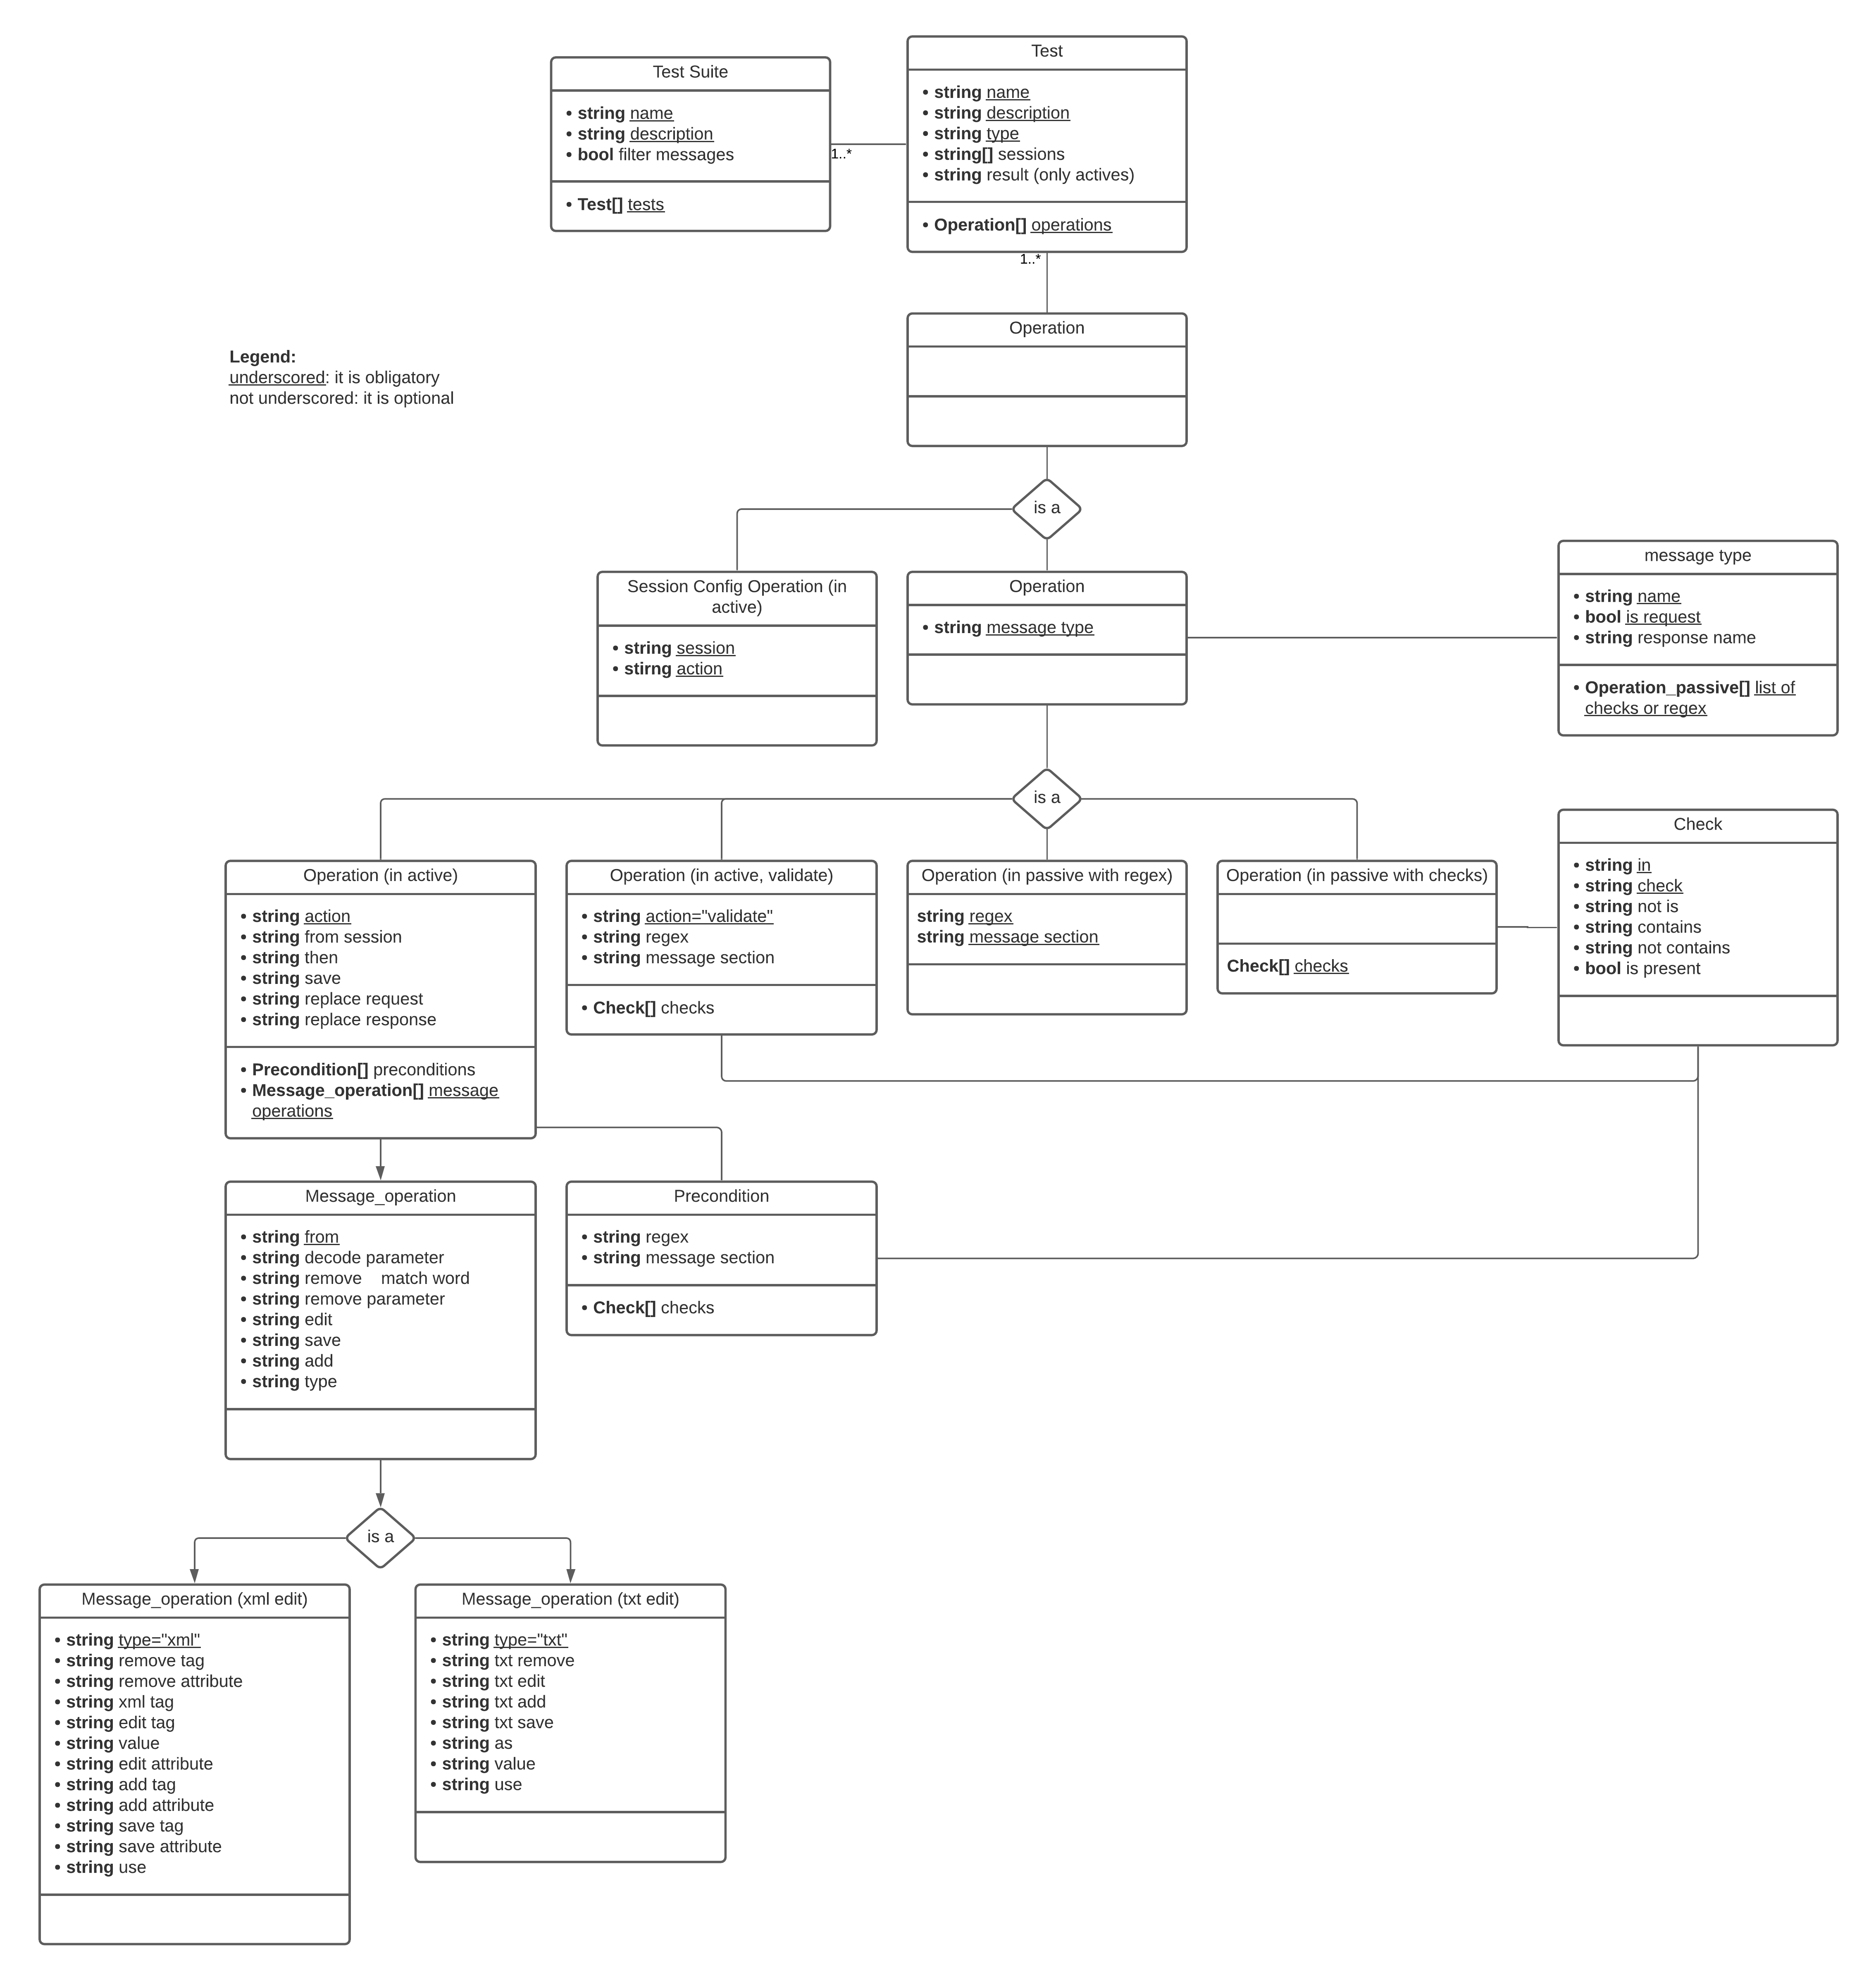
\includegraphics[width=\textwidth]{language_structure.png}
    \caption{language structure}
    \label{fig:language_structure}
\end{figure}


\subsection{Test suite}
The test suite is the main Object which contains all the other one, it has these tags:
\begin{itemize}
    \item name, the name of the test suite
    \item description, the description of the test suite
    \item tests, which is a list containing the tests to be executed
\end{itemize}
Reffering to the test example above, the definition of the test suite for it is:

\begin{lstlisting}[language=json]
{
    "test suite": {
        "name": "OAuth active tests",
        "description": "A test suite containing a OAuth test"
    },
    "tests": [
        {
            // A test
        }
    ]
}
\end{lstlisting}

As we can see, the Test Suite Object is a JSON object having the tag "test suite", with name and description, and a tag "tests" which will contain a list of Test Objects.

\subsection{Test}
Following the gerarchical order, the Test object is the one that actually defines a test. As said earlier, a test is contained in a Test Suite, and has various tags to be defined:
\begin{itemize}
    \item name
    \item description
    \item type, it can be "active" or "passive"
    \item sessions, which is a list of the sessions which are needed in this test
    \item result, (only for actives) it defines the conditions over which the test is considered passed or not.
    \item operations, a list of Operation objects which will be executed.
\end{itemize}

A test can be defined either as active or passive depending on the type of actions it has to do on the intercepted messages. If a test doesn't need to manipulate the flow or the content of the messages is considered passive, otherwise it is considered active.
The list of Operation Objects contained in a Test is executed iteratively one after the other. Only after the actual Operation has finished the execution the next is started.

Following the PKCE example above, we define an active Test:

\begin{lstlisting}[language=json]
{
    "test": {
        "name": "PKCE Downgrade",
        "description": "Tries to remove code_challenge parameter",
        "type": "active",
        "sessions": [
            "s1"
        ],
        "operations": [
            // list of Operation Objects
        ],
        "result": "incorrect flow s1"
    }
}    
\end{lstlisting}

We define the test, specifying its type, which is active, as it has to edit a message removing a parameter from the url, we define a session to be used (more on that later in this chapter) and we add a list of Operation to be executed. The result of the test is also specified, this will also be discussed later in the chapter.

\subsection{Operation}
The Operation object is the component that defines what a test actually does. As shown in the language structure image \ref{fig:language_structure}, an operation could be either a standard operation or a session config operation, the latter is used to manage the sessions for the active tests (i.e. start, stop, pause them). Depending on the type of test which an Operation is defined into, the standard Operation becomes active or passive.
In both cases, an operation has to contain the \textbf{message type} which defines the type of message to be intercepted in that particular operation (more info in the dedicated paragraph).
\\A \textbf{passive} operation has as objective to verify the presence (or absence) of some text or parameters in the intercepted message, to do this, it should contain one of the following options:
\begin{itemize}
    \item A list of Check objects, which are then executed to check the presence (or absence) of some text or parameter
    \item A regex inspection, which executes an inspection considering the intercepted message as plain text and executing a regex over it, if the regex has a match, the operation is considered passed, otherwise failed. Note that when a regex is used, it has to be specified also the message section over which to execute it (boy, head, url)
\end{itemize}

If the Test where the operations are defined is an \textbf{active} test, also if the intercepted messages need to be manipulated in some way, an active Operation has to be defined. It is composed by:
\begin{itemize}
    \item action, the action it has to do (intercept, validate)
    \item from session, from which session to expect the message to be intercepted
    \item then, the action to to after the receiving and manipulation of the message (forward or drop)
    \item replace request (or response), specify a previously saved message in order to replace it to the intercepted one
    \item preconditions, a list of Precondition objects
    \item message operations, a list of Message Operation objects, which will do the actual manipulation of the intercepted message
\end{itemize}

If the action is set to "\textbf{validate}" the operation becomes like a passive operation, because its objective is just to verify that some messages are as wanted. It will contain or a regex or a list of checks to be done. The Validate Operation is part of the Oracle, that is the component that decides whether the tests should be considered passed or not, more details on Oracle section.

In the PKCE example above, we define an Operation Object for an active test. This Operation has to intercept the "authorization request" message from session "s1", it has to check some Preconditions over it and then do some Message Operations. At the end the message is forwarded. More details on preconditions and Message operations in the next sections.

\begin{lstlisting}[language=json]
{
    "action": "intercept",
    "from session": "s1",
    "then": "forward",
    "message type": "authorization request",
    "preconditions": [
        // Precondition list
    ],
    "message operations": [
        // Message Operation list
    ]
}
\end{lstlisting}

\subsection{Message Operation}
The message operation is the Object that actually does the manipulations on the intercepted messages. It is composed by these tags:
\begin{itemize}
    \item from, the message section to work on
    \item decode parameter (optional) it indicates which parameter or string to be decoded before processed
    \item encodings (optional) the list of encodings to be applied to the parameter or text to be decoded. The supported encodings are base64, deflate, url
    \item remove match word (optional), remove text from te specified section in the matched message, it uses a regex
    \item edit, edit the matched text
    \item save, (optional) used to save an entire message in a variable in a way it can be used in future operations
    \item add, (optional) add some text after the matched text
    \item type (optional) specify the type of edit you want to do over a decoded parameter
\end{itemize}

In a message operation there is the possibility to specify a parameter or some text to be decoded before manipulation, to do that, specify with "decode parameter" the parameter to be decoded and with "encodings" the encodings necessary to decode the parameter. The parameter (or text) decoded, at the end of the Message operation will be encoded again automatically.
The decoded parameter can be manipulated by means of the "\textbf{type}" tag, there is the possibility to intepreter the decoded parameter as plain text, and to edit it using some actions:
\begin{itemize}
    \item txt remove
    \item txt edit
    \item txt add
    \item txt save
\end{itemize}
All the previous tags accept a regex, and whatever that regex matches will be edited or added or saved based on the specified tag.

Another possibility is to interpret the decoded text as xml, assigning the type tag "xml".
This way we have various possible operations to be done on the xml:
\begin{itemize}
    \item remove tag
    \item remove attribute
    \item edit tag
    \item edit attribute
    \item add tag
    \item add attribute 
    \item save tag
    \item save attribute
\end{itemize}

In the PKCE example above, we have just a simple Message Operation which has to remove the parameter "code\_challenge" frome the url of the message, so the resulting Message Operation will be:
\begin{lstlisting}[language=json]
{
    "from": "url",
    "remove parameter": "code_challenge"
}
\end{lstlisting}

\subsection{Message type definition}
The message type definition is needed in order to define some types of message that will be later used in the language to intercept them.
The message type definition is not actually part of the language, but it is stored in a file in the burp folder. Anyway, the definition of the type of messages uses the same Objects as the language.
A message type object is defined using these tags:
\begin{itemize}
    \item name, the name that will be used in the language to refer to this message type
    \item is request, if set to true if the searched message is a request, false otherwise
    \item response name, the name that will be used in the language to refer to the response of the searched message
    \item checks, a list of Check objects used to identify the message. If evaluated to true, the message is considered found
\end{itemize}

This is an example that defines the SAML request and the SAML response messages
\begin{lstlisting}[language=json]
{
    "message_types": [
        {
            "name": "saml request",
            "is request": true,
            "checks": [
                {
                    "in": "url",
                    "check param": "SAMLRequest",
                    "is present": true
                }
            ]
        },
        {
            "name": "saml response",
            "is request": true,
            "checks": [
                {
                    "in": "body",
                    "check param": "SAMLResponse",
                    "is present": true
                }
            ]
        }
    ]
}
\end{lstlisting}
The SAML request message has in its url the parameter "SAMLRequest", the SAML response message instead, has the "SAMLResponse" parameter in the body. Then, if a saml request has to be intercepted in a test, it has to be defined in the message types, and then used in the Operation.
As a result, if "saml request" is used in an Operation, the message having the parameter "SAMLRequest" in his url will be intercepted and processed by the Operation.


\section{The oracle}
The ensemble of all parts of the language that decide the result of the tests is called Oracle,
the oracle decides whether a test should be considered passed or failed (or not applicable). I decided to build the oracle in a way that can be almost fully customized by the user. 
The oracle is based on three main components:
\begin{itemize}
    \item Evaluation of the complete (or incomplete) execution of the \gls{session track} 
    \item Evaluation of the Precondition objects
    \item Evaluation of the Validate objects
\end{itemize}
If all the above conditions are met, the test is considered passed, otherwise it is considered failed.
The oracle can be built for example by using Validate objects to verify that some intercepted messages satisfy some conditions like having a particular parameter or string in them.

From the PKCE example above, both the result of the test and the precondition as been used:
\begin{lstlisting}[language=json]
"preconditions": [
    {
        "in": "url",
        "check param": "code_challenge",
        "is present": true
    }
],
\end{lstlisting}
With this precondition, the test has to be considered "not applicable" if the parameter code\_challenge is not found in the authorization request message. This means that is not possible to execute the given test over the actual intercepted message if the preconditions are not satisfied.
The result tag of the Test in the PKCE example is set to:
\begin{lstlisting}[language=json]
"result": "incorrect flow s1"
\end{lstlisting}
this means that the oracle will evaluate the test as passed if and only if the execution of the \gls{session track} of the session s1 will be incorrect, this means that if the browser will encounter some type of page which was not meant to encounter, the test will be considered passed. With "was not meant to encounter" I mean that the actions in the \gls{session track} cannot be done, because the objects that should be pressed in the page are not present, this happens for example if an error page is displayed, which tells us the service is not vulnerable to the Test, so the test is passed.

\section{Sessions}
A session is a browser executing a \gls{session track}, which is a list of user actions that the browser will execute automatically during execution of the Tests. There is the possibility of defining and using more than one session, in a way that (i.e.) reply tests can be executed.
As said in the previous sections, a "from session" tag can be specified in the Operation, this will tell in which of the available session search the desired message. To define the \gls{session track} I have used and extended the idea used in \cite{giulio_pellizzari}\cite{claudio_grisenti}\cite{stefano_facchini}, adding some options like "wait" and "clear cookies" functionalities.
The syntax of the \gls{session track} is based on the plain text export of Katalon Recorder\cite{katalon_recorder_syntax}.
An example of a \gls{session track} that does the login at unitn.it:

\begin{lstlisting}[]
    open | https://www.google.com/ |
    click | id=L2AGLb |
    click | link=Accedi |
    click | id=identifierId |
    type | id=identifierId | matteo.bitussi@studenti.unitn.it
    click | id=identifierNext |
    click | id=clid |
    type | id=clid | matteo.bitussi@unitn.it
    click | id=inputPassword |
    type | id=inputPassword | password
    click | id=btnAccedi |
    click | link=Gmail |
\end{lstlisting}

This \gls{session track} will do the login on the Unitn website using some credentials and password. The supported actions are:
\begin{itemize}
    \item open $|$ url $|$, to open an url
    \item click $|$ id=, link=, xpath= $|$, to click on a http object with the given id, link or xpath
    \item type $|$ id= $|$ text, to write on a given http element the given text
    \item wait $|$ milliseconds, to make the execution of the session wait for a given time 
    \item clear cookies $|$, to make the browser of the session clear all of the cookies in it
\end{itemize}



